\documentclass[10pt]{article}
\usepackage{acl2014}
\usepackage[utf8]{inputenc}
\usepackage{times}
\usepackage{url}
\usepackage{amsmath}
\usepackage[natbib=true,backend=bibtex,style=authoryear,language=english]{biblatex}
\usepackage{lipsum}
\usepackage{latexsym}
\usepackage[normalem]{ulem}
\usepackage[ruled]{algorithm2e}
\usepackage[]{setspace}
\useunder{\uline}{\ul}{}
\usepackage{caption} 
\usepackage{lastpage}
\pagestyle{plain} 
\usepackage{graphicx}
\captionsetup[table]{skip=10pt}
\title{Intelligent Traffic Control}

\addbibresource{references.bib}
\AtBeginBibliography{\small}

\author{Thomas van den Broek, Vincent Van Driel, Zsolt Harsányi, Tonio Weidler\\
	Department of Data Science \& Knowledge Engineering\\
	Maastricht, The Netherlands\\
	\tt \small vincevandriel@gmail.com, thomasbuo@gmail.com,\\
	\tt \small zsharsany@gmail.com, uni@tonioweidler.de
}
  
\begin{document}

\maketitle
\begin{abstract}
\lipsum[1]
{{\it \bf Keywords:} traffic simulation; traffic control; strategies; linear programming; machine learning; realistic environment; IDM; MOBIL;}
\end{abstract}

\section{Introduction}
An intelligent traffic control system adjusts traffic in order to assure all people reach their destinations in the most optimal time and distance. These systems are important for the daily workings of major cities by alleviating traffic congestion and identifying problematic areas. It is important to constantly keep these systems updated to assure optimal performance and safety of the general public. With advancements in technology and artificial intelligence, new and more sophisticated strategies for traffic control become possible.

\subsection{Research Questions}
This work aims to evaluate various traffic control strategies and compare their effect in different scenarios. In particular, we aim to investigate, whether different traffic signal control strategies are best suited for different street layouts or if there is the latter induce consistent rankings. Furthermore, experiments are conducted in order to compare the effectiveness of strategies controling the behaviour of traffic signals and such that are related to urban planning, e.g. introduction of new lanes or entirely new roads.

\subsection{Approach}
Hence, in order to test the effect of different intelligent traffic control strategies, an appropriate simulation is required. For this purpose, we created a simulation environment which allows the incorporation of different such strategies into a dynamic traffic model. Our simulation aims to model the dynamics of a realistic environment as close as possible within the scope of the project, so that the comparison is meaningful and provides valuable data regarding the potential application of the strategies. The simulation is \textit{microscopic}. That is, instead of globally controlling traffic (\textit{macroscopic}), the atomic parts of the simulation are locally controlled cars \citep[see also][]{krajzewicz2002sumo}. Driving behaviour is modelled using the time- and space-continuous \textit{Intelligent Driver Model} (IDM) \citep{treiber2000congested}. We make our code publicly available at GitHub\footnote{https://github.com/weidler/traffic-simulation}.

\subsection{Related Work}
\label{sec:related-work}
In the following, previous research on this topic will be briefly summarized. There has been extensive work on the simulation of traffic flow as well as the development of traffic control strategies. Following up on different approaches on modelling car following behaviour \citep[e.g.][]{gipps1981behavioural}, \citet{treiber2000congested} developed the influential \textit{Intelligent Driver Model} for the simulation of urban traffic. Similarly to the former, it creates a collision free environment where cars mind the  spacial and time-wise gap to the leading vehicle. The SUMO package \citep{krajzewicz2002sumo, behrisch2011sumo} utilizes the model by \citep{gipps1981behavioural} in an extended version \citep{krauss1998microscopic} in a complex simulation software. In contrast to their research, this work uses the IDM. Hence, the simulation is time-continuous, rather than time-discrete.

Often utilizing such simulation environments for evaluation purposes, a lot of research exists investigating the strengths of different approaches to the automatic control of traffic signals or traffic lights. \citet{papageorgiou2003review} have reviewed such research and identified two key characteristics according to which strategies may be classified. They distinguish between \textit{fixed-time} and \textit{traffic-responsive} strategies, as well as \textit{isolated} and \textit{coordinated} strategies. Fixed-time strategies use historical data to determine (e.g. by optimization) static cycle lengths, while traffic-responsive strategies may use different techniques (e.g. heuristics or optimization algorithms) in order to derive optimal cycle lengths from real-time data that has to be measured in some way. Isolated strategies are focused on a single intersection, while coordinated strategies are able to communicate information between multiple intersections and thereby make potentially joint decisions. \citet{coll2013linear} categorize strategies into four categories. They also distinguish between fixed-time and traffic-responsive approaches, but additionally differentiate \textit{adaptive systems} that apply optimization techniques and \textit{predictive strategies} that use both online and off-line information in order to predict future arrivals at the intersection \citep{coll2013linear}. In this work, the focus will be laid on the former two categories, that is, fixed-time and responsive.

The linear programming (LP) optimization was an attempt to optimize the duration of cycles for traffic lights using predictions based on the queue size at red and green lights, flow capacity, and cycle length from the previous time step.  As the incoming traffic density from each road entering an intersection changes, the length of green and red phases for the corresponding traffic light is gradually adjusted to assure an optimal output flow.  Using the LP strategy in conjunction with some other traffic control strategies, such as the weighted strategy, was predicted to further optimize the performance of the strategies as well as making the adjustments more smoothly than the traffic control strategies by themselves.

\vspace{20pt}

In the following sections we further describe our approach and the results of our experiments. We begin by elaborating on the implementation of the simulation environment (section \ref{sec:envi}), followed by a description of different control strategies (section \ref{sec:strategies}). Following, we describe the experiments we conducted for those strategies and our evaluation methodology (section \ref{sec:experiments}). In section \ref{sec:results} we will report the results of these experiments. We conclude this work by discussing our results and proposing future directions.
	
\section{Simulation Environment}
\label{sec:envi}
In the following subsections we describe the implementation and design choices of the simulation environment in which we evaluated the effect of different traffic control strategies.
	
\subsection{Traffic Flow Simulation}
As mentioned beforehand, the IDM \citep{treiber2000congested} is applied for the simulation of car dynamics. It models traffic flow time- and space-continuous as a combination of \textit{free-road} and \textit{interaction} behaviour. The \textit{free-road term} is governed by a car's intention to reach its desired speed. The acceleration for this behaviour is calculated \citep{treiber2000congested} as

\begin{equation}
	\label{eq:free-road-term}
	\dot{v}_a^{\mathrm{free}}(t) = a ( 1 - ( \frac{v_a}{v_0} )^\delta),
\end{equation}

where $a$ refers to a cars maximum acceleration, $v_a$ is its current velocity and $v_0$ the desired velocity. When a car approaches a leading vehicle, it is supposed to slow down in order to avoid collision. This behaviour is modelled by an \textit{interaction term} which incorporates the distance to the leading vehicle and its speed \citep{treiber2000congested}. 

\begin{equation}
	\label{eq:int-term}
	\dot{v}_a^{\mathrm{int}}(t) = - a ( \frac{s_0 + v_a T}{s_a} + \frac{v_a \Delta v_a}{2 \sqrt{ab} s_a} )^2
\end{equation}

In the equation above, $s_0$ and $T$ restrict the cars minimum distance in space and time respectively. The interaction term will hence attenuate the free road term when approaching other cars, given by the complete equation for acceleration $\dot{v}(t)$

\begin{equation}
	\dot{v}(t) = \dot{v}_a^{\mathrm{free}}(t) + \dot{v}_a^{\mathrm{int}}(t)
\end{equation}

In order to simulate a time-continuous model, we need to numerically approximate the integration of the differential equations in \ref{eq:free-road-term} and \ref{eq:int-term}. For that, we choose a small time step $\Delta t$ and repetitively update the velocity as $v(t + \Delta t) = v(t) + \dot{v}(t)$.

\subsection{Traffic Rule Compliance}
Due to the large scale maps used in this work, drivers not only need to behave according to their own desires and other traffic participants. They additionally need to comply to a set of traffic rules as given by speed limits or traffic lights. Following, we briefly discuss the approaches we use in our simulation.

\paragraph{Approaching Traffic Lights} When approaching red traffic lights, drivers will stop in a predefined distance from the intersection, comparable to stop bars in real world streets. Cars that have already exceeded this line will drive through the intersection. 

\paragraph{Speed Limits} The IDM's free road term incorporates a driver's desired velocity as his intended maximum speed. We use an additional parameter, a driver's favoured velocity $v_{fav}$, and determine the desired velocity by taking the minimum of $v_{fav}$ and the roads speed limit.

\subsection{Lane Changing}
In order to incorporate lane changing behaviour into our traffic model, we apply the MOBIL model \citep{treiber2002realistische, kesting2007general}. MOBIL makes decisions for lane changing based on two questions: Is the lane change \textit{incentive} and is it \textit{safe}? The former question is answered based on the potential gain in acceleration on the new lane, while the latter decision is made based on the speed of and distance of the approaching car on the new lane.

\subsection{Arrival Times in a Continuous Simulation}
Rather than predefining arrival times for a fixed simulation duration, we dynamically generate inter-arrival times (IAT) during runtime. These IATs are drawn from a predefined distribution independently for each road in the map. Therefore the amount of traffic on a map grows automatically with its size. The IAT can be drawn from the following distributions

\begin{figure}[t]
	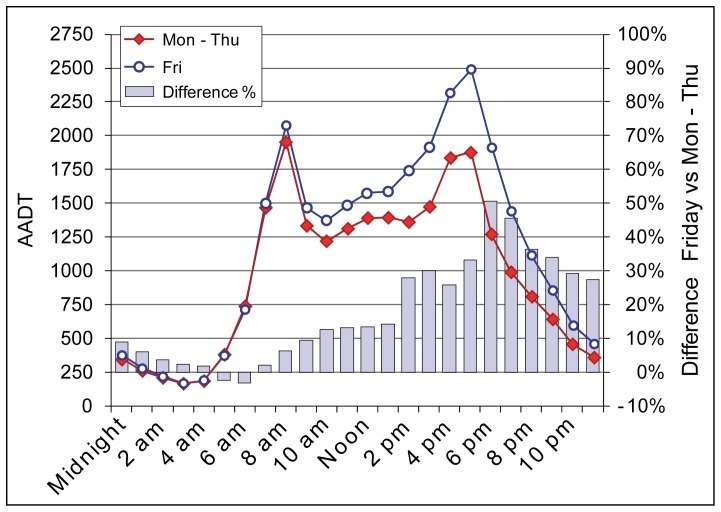
\includegraphics[width=\linewidth]{img/traffic-data.jpeg}
	\caption{Traffic data from the U.S. Department of Transportation. Graphic received from https://www.fhwa.dot.gov/policyinformation/tmguide/
	tmg\_2013/traffic-monitoring-methodologies.cfm \label{fig:traffic-data}}
\end{figure} 
 
\begin{itemize}
	\item Exponential (Poisson Process)
	\item Gaussian
	\item Realistic (Non stationary Poisson Process)
\end{itemize}
 
While the Gaussian and Exponential distribution are standard distributions with adjustable paramters, the realistic distribution is based on real world data from the U.S. Department of Transportation \citep{trafficdata}. We use hourly data and draw IATs based on a poisson process that is then fitted to the data using the thinning algorithm by \citet{lewis1979simulation}. The data used is shown in figure \ref{fig:traffic-data}. As can be observed, this creates rush hours around the hours of 8 to 9 am and 5 to 6 pm.

\subsection{Path Finding}
Whenever a car enters the traffic, it needs to get a predefined route to take to its destination. In the simulation, each car runs an instance of a path finding algorithm, two of which were implemented.

\paragraph{A*}
This popular path finding algorithm, based on Dijkstra’s algorithm \citep{dijkstra1959note}, was first introduced in 1968, by \citet{hart1968formal}. It finds the shortest path between the origin and the destination of the cars, given the map only taking the length of the path into account. This is done by using two scores for each node: H and G score. The H score is equal to the Euclidean distance from the node to the destination. The G score is the total distance travelled from the start node to the current node. Based on these two scores, the algorithm finds the shortest path between two points in a graph. 

\paragraph{Advanced A*}
The advanced A* path finding algorithm is very similar to the original version, but it also takes the traffic density and average speed of the roads into account. This is realized by calculating the traffic density and average speed of each road whenever the route of a car is created. The density of a road equals the number of cars on it divided by the length of the road, to get the number of cars per meter of road. The algorithm then adds a weighted density value to the G and H scores of the road to calculate the current best route. The average speed for the roads is taken from the continuously calculated statistics. The value of the average speed is taken away from the score of the road, in order to incentivize the use of roads with a higher speed.

\subsection{Zone-based Scheduling}
Aiming to increase the level of realism, roads on the simulated map have different types of zones that influence the spawn rates and routing of cars. Distinguished zones are \textit{residential}, \textit{mixed}, \textit{commercial} and \textit{industrial}. A road's zone restricts its \textit{available population} in the beginning of the simulation. For instance, commercial zones start with a lower overall population than residential zones. Cars will only spawn from roads as long as there is population available. Whenever a car leaves or arrives at a road, its population is respectively decremented or incremented. Additionally, the zone type determines the traffic flow between different areas of the map. Based on the time of day, cars either mostly move from residential and mixed zones to industrial and commercial zone or vice versa, when they are on their way back home. This way, the simulation also incorporates the difficulties of heavy traffic in one direction, as faced in cities where living and working places are seperated by its different areas. Figure \ref{fig:zone-traffic-flow} sketches how the traffic behaves between the zones based on the time of day.

\begin{figure}
	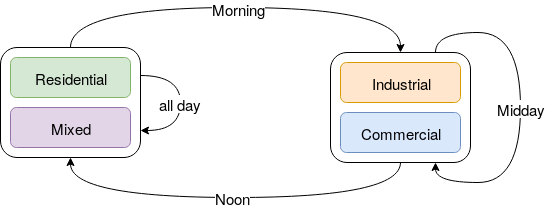
\includegraphics[width=\linewidth]{img/zoned-traffic-flow.png}
	\caption{Traffic Flow between different zone types at different times of the day. \label{fig:zone-traffic-flow}}
\end{figure}

\subsection{Simulation Model}
Putting the above parts together, the simulation procedure depicted by algorithm \ref{alg:simulation} is run.

\DontPrintSemicolon
\setstretch{1.2}
\begin{algorithm}[h]
	\;
	\KwData{Map m, CarList c, Schedule s, days d, delta\_t}
	\;
	\textit{Initialize} trafficlights\;
	\textit{Initialize} tracking variables\;
	\; 
	\While{simulated\_days $<$ d}{
		\textit{update} time\_parameters\;
		\;
		\ForEach{Road r in m}{
			\If{r.nextArrival == now}{
				\textit{spawn} car\;
				r.availablePopulation--\;
				\textit{generate} nextIAT\;
			}		
		}
		\;
		\textit{update} trafficlights\;
		\textit{update} car positions \textit{and} velocities\;
		\textit{remove} arrived\_cars \textit{and} adjust population\;
		\;
		\textit{visualize}\;
		\textit{track} statistics\;
	}
	\;
	\textit{report} statistics\;	
	
	\caption{Simulation procedure. \label{alg:simulation}}

\end{algorithm}
\setstretch{1}

\section{Traffic Control Strategies}

\begin{figure*}[htb]
	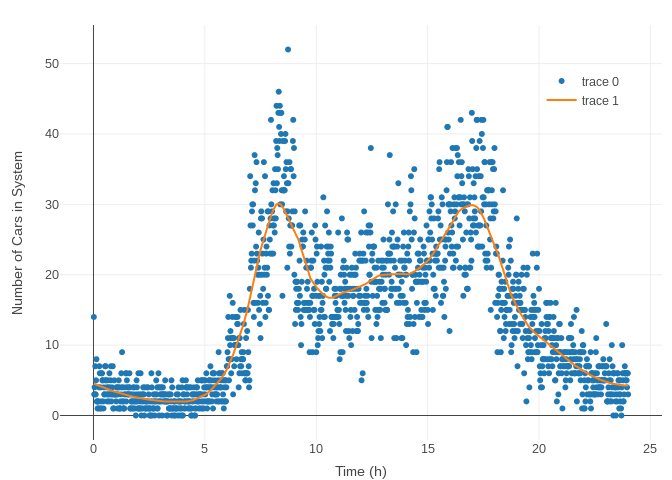
\includegraphics[width=0.5\textwidth]{img/number_of_cars_over_day.png}
	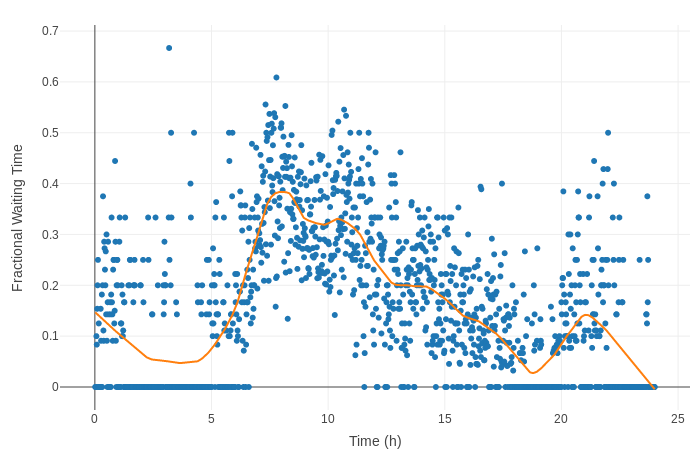
\includegraphics[width=0.5\textwidth]{img/velocity_over_day.png}
	\caption{Number of cars (left) and average velocity of cars (right) in the system simulated for one day. IATs are generated from the empirical distribution shown in figure \ref{fig:traffic-data}. \label{fig:validation}}
\end{figure*}

\label{sec:strategies}
In this section, different traffic control strategies are highlighted as well as their effectiveness in different environments.

\subsection{Benchmark Strategies} 
In order to provide a baseline of what more advanced strategies should be able to outperform, we implemented two simple benchmark strategies. The first one is \textbf{Basic Cycling} and refers to a traffic light control strategy based on a simple, fixed-time cycle in which one traffic light at a time is green. The second is \textbf{Informed Cycling} and refers to a similar strategy, in which a road's green phase is skipped if there are no cars waiting on it.

\subsection{Responsive Strategies}
\label{sec:responsive}
These strategies should outperform the benchmark strategies as they are more dynamic and change their actions based on their surroundings. Weighted Cycling intends to reduce the time people spend waiting at a light. Simply put, the traffic lights give priority to those who are waiting at the light, and if no one is waiting, it gives priority to the street with the most cars incoming. This method seems to mimic real-world examples of traffic control systems by acting similar to a traffic light with some form of traffic sensors (pressure plates, traffic cameras, etc.). It also allows the most amount of people possible through fastest, which is extremely effective in situations where a large amount of cars approach from one side. 

Additionally, three strategies are investigated that, similarly to \textit{Basic Cycling}, choose the next green light in a given order. Crucially though, they do not use fixed times for the green phase. Instead, the phaselength is determined by some strategy-specific measure of traffic, normalised by the total traffic surrounding the intersection.

\paragraph{Density Weighted Cycling} The most simple of such strategies uses the total number of cars that come from a road to determine the phaselength of the traffic signal. It therefore assigns longer phaselengths to trafficlights that have more cars approaching the intersection relative to all other incoming roads.

\paragraph{Queue Weighted Cycling} Aiming to more precisely judge the severity of traffic load incoming from a road, this second weighting approach only takes into account cars that are actually waiting at a traffic light. A car is classified as waiting if it is slower than $5\ km/h$ and has a negative acceleration.

\paragraph{Flow Weighted Cycling} Finally, the last of such strategies weights by taking into account the traffic flow coming from a road during its previous green phase. Thereby, roads are preferred that predictively enqueue the most cars when turned green. The most apparent advantage of this approach is the fact that it will not give too much attention to overfilled roads that can actually not be relieved when lights turn green because the following traffic disallows it.

\paragraph{Dynamic Strategies} Dynamic strategies are strategies that instead of deciding how long a light has to stay green decides which light to turn green based on the information that the intersection gathers. Currently there are two strategies that do this.

\paragraph{Dynamic Cycling (WEIGHTED)}

The first strategy that determines which light of an intersection should turn green is Dynamic Cycling. This strategy measures the amount of cares that are moving towards the intersection for each connected road and chooses to turn the light green for the road which has the most incoming traffic. It makes the next decision at a set interval.

\paragraph{Dynamic Cycling+ (COORDINATED)}

The second strategy is Dynaminc Cycling+. This strategy is a more advanced version of the regular Dynamic Cycling. The differenc is that Dynamic Cycling+ does not only measure the incoming traffic for each road but also measures their average speed. it chooses to turn the light green for the road with the lowest average speed. Should the average speed of two or more roads be close to each other, then the intersection will choose the road with teh most incoming traffic. Another feature this strategy has is that at every traffic light has to turn green at least once within a certain amount of time. This is to prevent some roads from never turning green and thus causing some cars to never be able to drive.

\section{Methodology \& Experiments}
\label{sec:experiments}

\subsection{Measured Statistics}
In order to be able to measure and compare the efficiency of the different strategies applied, various measurements are taken while the simulation is running. One of these is the average speed of the vehicles for each road. Measuring this is done by starting a timer for a car when it enters a road and stopping it when it leaves it. Then, by using the following formula, the average speed is calculated:   

\begin{equation}
	v = \frac{s}{t}
\end{equation}

where $v$ is the velocity, s the road length and t refers to the time spent on a road. Using this, we can also easily derive the average speed on each road. The second statistic measured is the amount of time each car spends waiting at traffic lights. This is achieved by checking at each time step if a car is under a certain speed and is not accelerating. Whenever the previous conditions are fulfilled, the total amount of waiting time is increased by the size of the time step. The purpose of the control strategies is to maximize the average speeds and minimize the time spent waiting in congestions.

\subsection{Simulated Maps}

\paragraph{Two Districts}

\paragraph{Chaos City}

\paragraph{Brusselsepoort}

\paragraph{Tie Fighter}

\subsection{Simulation Validation}
In order to validate both the IA generation as well as the general behaviour of different measures and dynamics, we validated the simulation environment using the average speed of cars, their number on the map as well as fractional waiting times in the simulation as a development over one day. Figure \ref{fig:validation} shows the results in three graphs. As can be observed, not only the density, but also both other dependent measures resemble the rush hour pattern from the original data.

\subsection{Methodology}
It is the objective of this work to compare multiple systems (i.e. strategies) under different conditions. Since it is desirable in such a setting to not only compare these systems with a baseline or benchmark system but rather rank them by performance, a convenient framework for such a comparison is needed. An all-pairwise comparison is not desirable, since the total of  systems would require 30 comparisons, which would result in tiny confidence levels due to Bonferroni inequality \citep[see e.g.][]{law2007simulation}. Instead, the sample size required for each system in order to achieve a confidence level of $\alpha$ for the complete ranking can be determined by the approach of \citet{dudewicz1975allocation}. In order to perform statistical calculations on the data, it is often necessary but at least useful to have IID observations. It is obvious that this independence can not be assumed in a traffic simulation between individual cars, since the delay of one car often influences that of others in shared roads and queues. While restarting the simulation $n$ times in order to get $n$ observations that can be combined to a grand mean seems an obvious choice, the day-based simulation also allows to run multiple days and assume independence between days, since traffic is supposed to somewhat reset during night.

Since this is a non-terminating simulation, it is furthermore necessary to take a so called \textit{warm-up period} or \textit{transient phase} into account. It is the result of starting the simulation in an initial state that might not represent an actual state of the simulation in steady-state or inside a cycle. Therefore, the period where the simulation enters the steady-state needs to be removed from any statistical calculation such that it does not bias their results to the initial situation. Arguably, simulating traffic on the basis of days results in a cyclic simulation. Importantly though, this will not necessarily mean that the simulation entirely resets to zero cars in the system at midnight. For those reasons and the sake of convenience, in any experiment, the first simulated day will be removed from the simulation.

Three measures are employed to compare the performance strategies. Similarly to prior work CITE, the average velocity of cars in the system is measured. Additionally, we report the number of cars on the map and the percentage of cars waiting (as defined in section \ref{sec:responsive}).

\section{Results}
\label{sec:results}
In the following section, results for all experiments are presented. Firstly, the outcome of the optimization of the phase length parameter are reported and shortly discussed. Secondly, for each street layout, the performances of all strategies will be used to rank them. In the last subsection, the influence of some urban planning measures will be investigated.

\subsection{Phase Length Optimization}
Experiments for the optimization of phase lengths in all strategies were conducted on the Brusselsepoort map with 5 different configurations each and a simulation duration of 21 days (where the first day was removed as the transient phase. As the measure to be optimized on, we choose the average speed, since this is one of the most common metrics in the literature. Results of those experiments for the basic, informed and flow weighted strategy can be found in figure \ref{fig:opt-results} in the form of box plots as an average during the rush hour between 7 and 9 o'clock.

\begin{figure*}[t]
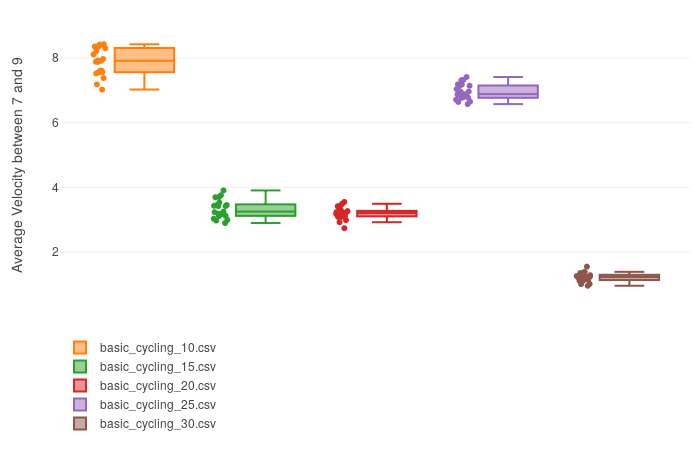
\includegraphics[width=0.5\textwidth]{img/basic-opt.png}
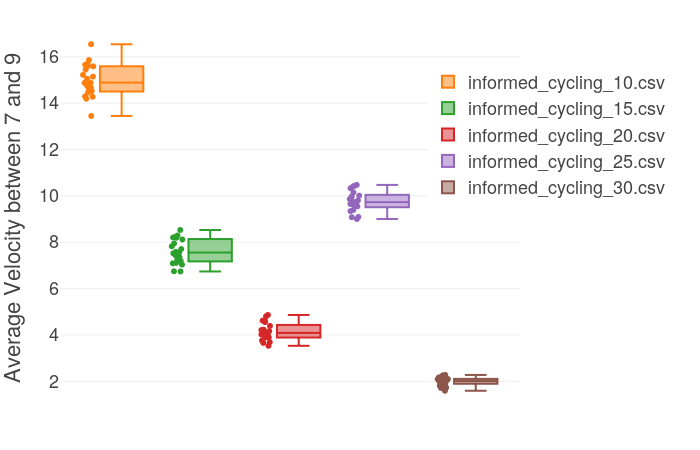
\includegraphics[width=0.5\textwidth]{img/informed-opt.png}
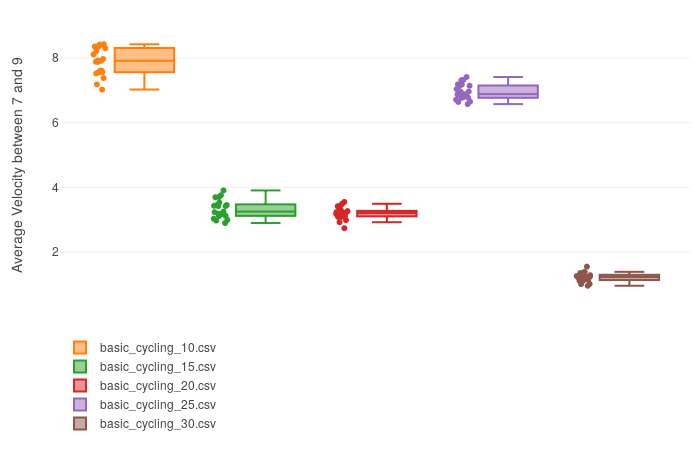
\includegraphics[width=0.5\textwidth]{img/basic-opt.png}

\caption{\label{fig:opt-results}}
\end{figure*}

As figure \ref{fig:opt-results} shows, in both basic and informed cycling, 10 seconds and 25 seconds are respectively the best and second best performing strategies numerically. Since 10 seconds is a rather low phase lengths which might get its benefits from the specific design of the simulation environment, we choose 25 seconds as the phase length for these two strategies in the following experiments.

\subsection{Relative Ranking of Strategies}

\subsection{Urban Planning}

\subsubsection{Introducing More Lanes}

\subsubsection{One Way Roads}

\section{Discussion}
\label{sec:discussion}

\section{Conclusion}
\label{sec:conclusion}

%- Often times, better road layout makes way more of a difference than different strategies (tiefighter example)

{\tiny\printbibliography}

\end{document}